\section{Approach}
\label{sec:approach}
This study investigates the potential of combining static analysis tools with \aclp{llm} to enhance the detection of software vulnerabilities while addressing the issue of false positives. 
The methodology involves using two static analyzers, CodeQL and Infer, to flag vulnerabilities, enriching their output with additional code context obtained through a code graph of the project, and leveraging an \ac{llm} to refine the results. 
Figure~\ref{fig1} provides an overview of the workflow.

\begin{figure}
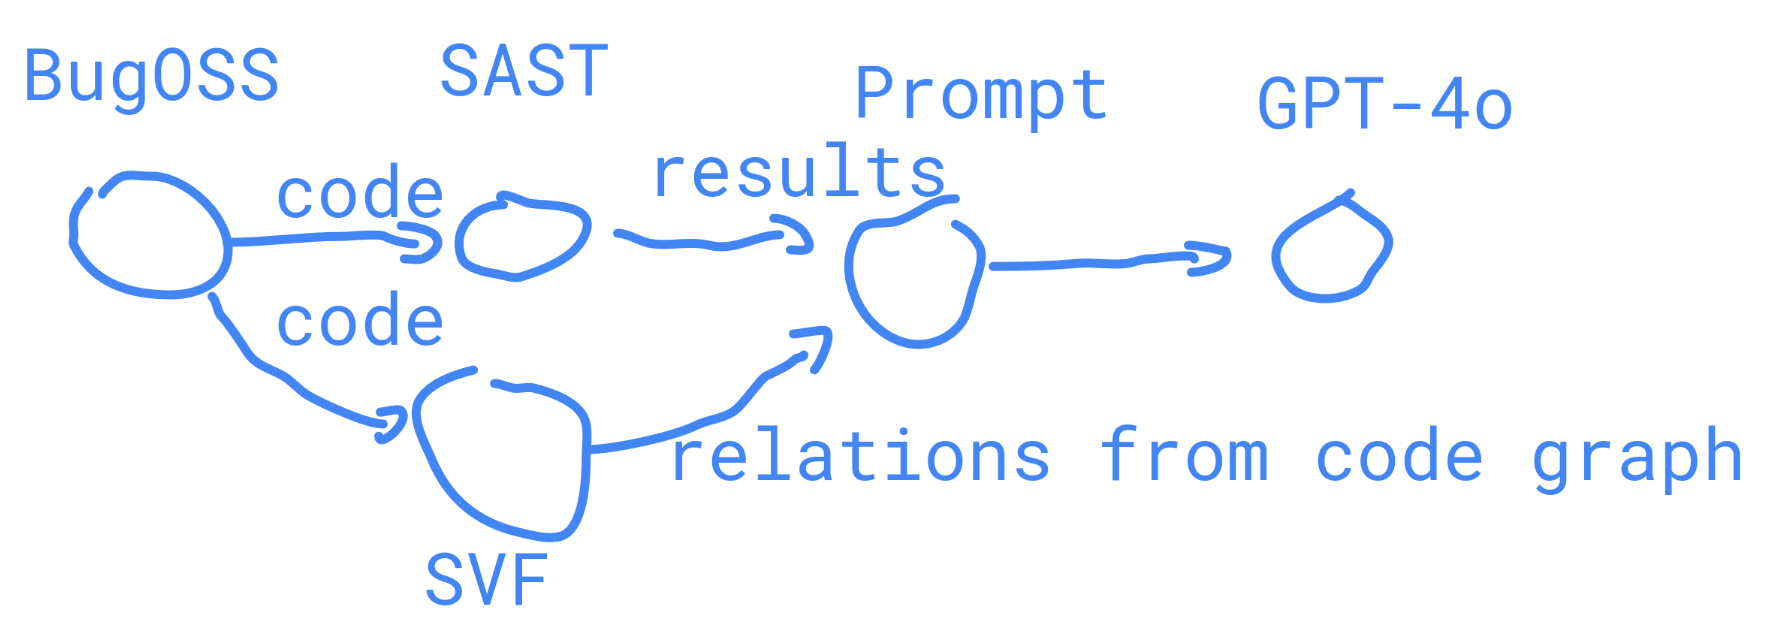
\includegraphics[width=\textwidth]{figures/fig1-workflow.png}
\caption{This diagram denotes the flow of information throughout the project.} 
\label{fig1}
\end{figure}

In each of the following subsections, detailed explanations of the tools used will be provided, with the goal of clarifying the diagram illustrated above step by step.

\subsection{Dataset and Ground Truths}
\label{sec:approach:sub:dataset}
BugOSS~\cite{BugOSS} is a dataset containing vulnerabilities manually detected in various \acl{oss} projects.
It comprises a total of 21 different real-world projects, ranging from lesser known projects like Poppler~\cite{poppler}, a library used for rendering PDFs, to widely used software tools, such as Curl~\cite{curl}, a command-line tool that enables data transfer with URLs.

Despite being originally crafted for examinations through fuzz testing, BugOSS contains, for each of the listed projects, information regarding the \ac{bic}, as well as the \ac{bfc}. Together with corresponding Dockerfiles and build scripts for each one of the projects, this dataset proves very useful for the reproducibility of the detected vulnerabilities.

\subsection{Static Analysis with CodeQL and Infer}
\label{sec:approach:sub:sast}
For the static analysis, two widely used tools were chosen: CodeQL and Infer.

\subsection{Contextual Analysis with SVF}
\label{sec:approach:sub:context}
To attain contextual information about the flagged vulnerable functions, the chosen method was to find out which other functions were callers and callees of the ones analyzed.
For this to be possible, it was necessary to generate and analyze the call graph of the code. 
A call graph is a different representation of a program, in which the program is depicted as a control-flow graph. 
In this form, each function becomes a node, and the relationships between functions, as in how they call one another, are shown as edges between the nodes.
Thus, this form facilitates the finding out of contextual information for the vulnerable functions.

To generate this call graph, SVF (Static Value-Flow Analysis Framework for Source Code) \cite{svf} was used. 
SVF is a code analysis tool enables interprocedural dependence analysis for LLVM-based languages. 
By providing SVF with a bytecode file generated with the LLVM compiler, this framework generates a .dot file describing the call graph. 

LLVM is an open-source compiler ...

An example of a .dot file is formatted and its translation into a graph illustration can be seen in Figure~\ref{fig2}

\begin{figure}
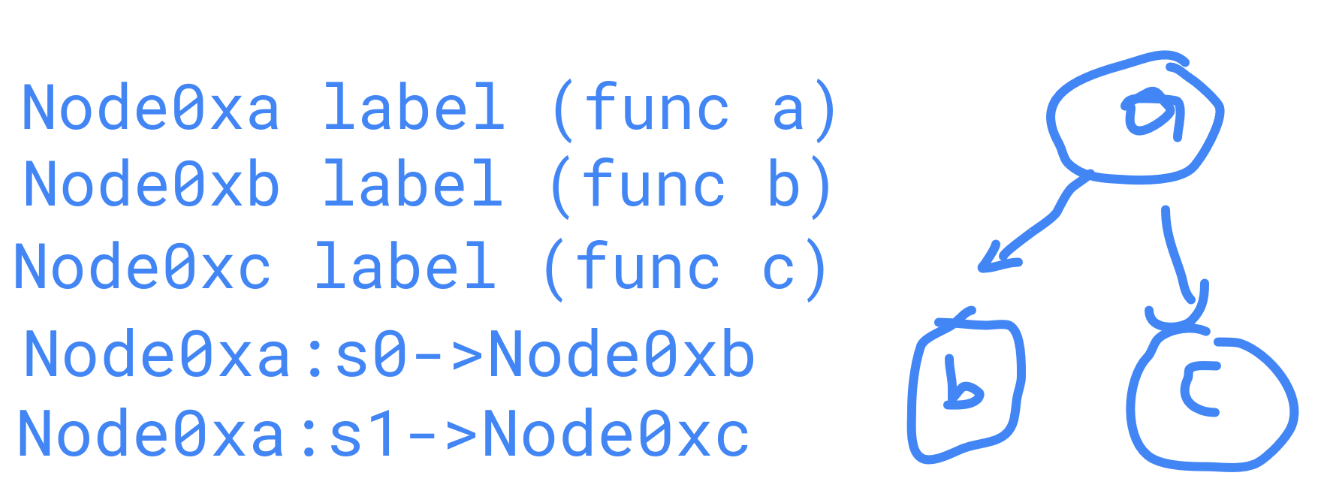
\includegraphics[width=\textwidth]{figures/fig2-callgraph.png}
\caption{This images show the side-by-side comparison of a node and its edge into dot-formatting with their graphical representation.} 
\label{fig2}
\end{figure}

After generating the call graph, it was necessary to filter out the vulnerable functions obtained as explained in Subsection~\ref{sec:approach:sub:sast}. 
This required at first a Python script to match the names of the functions with the corresponding labels of the nodes, as the nodes are not named directly after the functions, as depicted in Figure~\ref{fig2}. 
Some manual filtering was also required due to name mismatches.

The navigation of the graph for finding out callers and callees was done with the pydot~\cite{pydot} library, which easily handled the lookup of the relevant edges and connected functions.

\subsection{LLM Augmentation}
\label{sec:approach:sub:llm}
After attaining \ac{sast} results and the contextual information explained in the previous subsections, this data was then put together and formatted into a prompt.

The prompt was formatted as show in Figure 2:

\subsection{Summary}
\label{sec:approach:sub:summary}